\chapter{General}
\section{Overview}

The Campus Information System is the central web interface for students and staff. Various services are available here.
You can read the latest news, access information about the teaching and courses offered, look up teaching schedules and much more. 

\begin{figure}
	\centering
	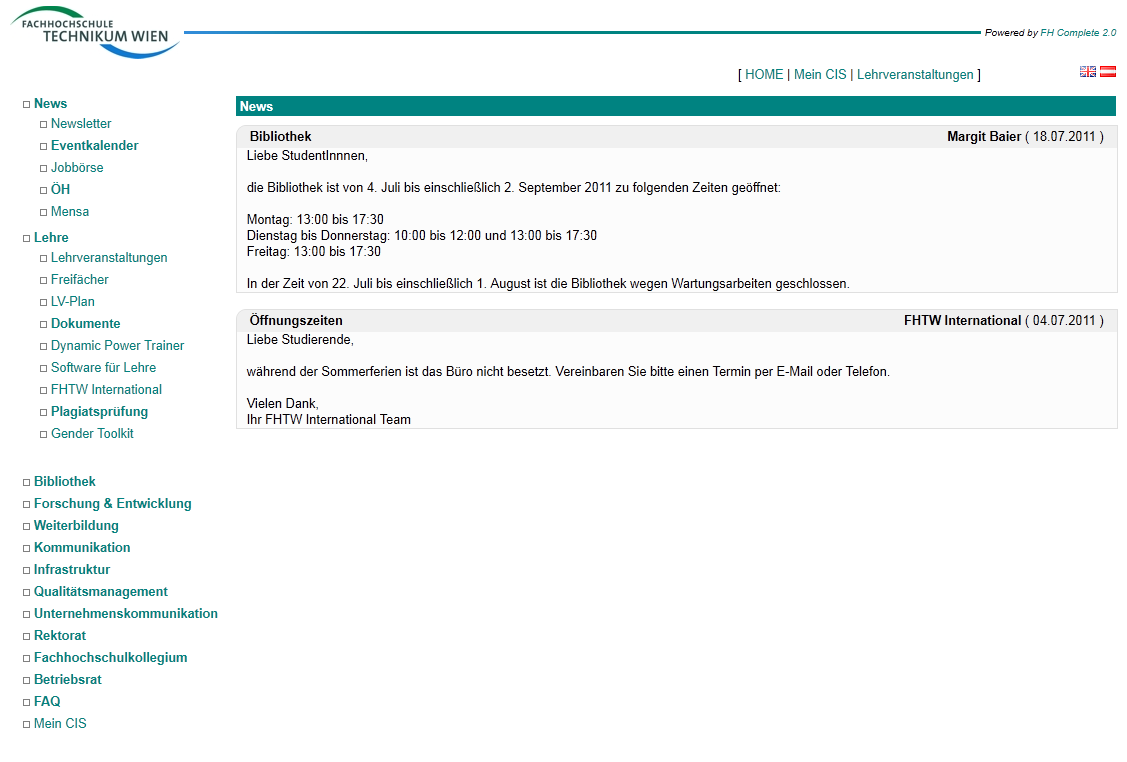
\includegraphics[width=0.70\textwidth]{CIS_Startseite.png}
	\caption{CIS HOME}
	\label{CIS_startseite}
\end{figure}

\section{Main Menu Sections}

	\minisec{News}
The CIS offers various news pages (also called Pinboard in the Course News section). The HOME page shows the view for "'General News"'. In addition, there are pages for each organizational unit (Degree Program, Institute,...). These are displayed on the appropriate sub-page together with the general news.
For the guidelines on managing news please see \ref{richtlinien_newseintraege}

The "'News"' section of the CIS also includes links to other external news and information platforms.

	\minisec{Teaching}
The Teaching section contains all the information and documents necessary for teaching, such as information about courses, attendance lists, grade lists, participant lists, mail groups, semester plan and the student upload tool to make carrying out exercises easier.

Furthermore, in this section you can also register for electives and find tools and information to help you with your teaching.
For more details, please see chapter \ref{lehre}.

	\minisec{Library}
Here you will find information about the library, research links, links to electronic media and external literature databases as well as the OPUS publication database.

	\minisec{Research \& Development}
In this section you will find information about ongoing projects as well as documents and procedures for conducting research projects.

	\minisec{In-service Training}
Here you can learn about which internal and external in-service training programs are currently being offered.

	\minisec{Communication}
Here you can view your contacts, webmail, UAS Technikum Wien mailing lists or search for a specific person.

	\minisec{Infrastructure}
The Infrastructure section contains the most important information about the technical and logistical infrastructure of the university:
Instructions and tools for connecting to the LAN and Wi-Fi networks, a free antivirus program, information about the media equipment available, maps, as well as regulations.

	\minisec{Quality Management}
Here you will find all the documents and processes relevant for studying at the UAS Technikum Wien, documents concerning the general organization of the UAS, as well as the relevant document templates.

	\minisec{Corporate Communications}
In this section you will find the UAS Technikum Wien company logo, corporate identity handbooks and an event guideline available for download.

	\minisec{Rector's Office}
Under "'Rector's Office"' you will find the UAS Technikum Wien mission statement, key figures, gender mainstreaming activities, university projects, awards and information on competitive tenders and grants.

	\minisec{University Council}
	In this section you will find a list of members and the rules of procedure for the Council of the UAS Technikum Wien, as well as the relevant documents.

	\minisec{Union Info}
News, information and important documents like internal agreements are available here.

	\minisec{FAQ}
The FAQ (frequently asked questions) section provides various instructions, solutions to common problems, handbooks, and a link to the archive.

	\minisec{My CIS}
In this section you will find all of your personal information as well as a number of administrative tools:
an overview of your profile data, your personal teaching schedule, preferred teaching times, the vacation tool (for staff), your courses (for lecturers) and tools for submitting Bachelor's and Master's theses.